%% Introducción
% El objetivo del proyecto es desarrollar un encriptador para asegurar las comunicaciones entre sitios.
% A -- B -- C

%% Motivación
% Problema de las soluciones comerciales (backdoors conocidos como CryptoAG).

% La diapo de plan de trabajo llevarla al inicio de Desarrollo.
%%%% Explicar/agregar lo que planificamos para este año.
% Marcar la diferencia entre la primera etapa y lo que sigue para este año. (Lo que hicimos en el primer semestre fue ENTENDER y hacer una arquitectura para la solución y un prototipo preliminar 100% software basado en hipervisor de tipo 2.)
% Para el segundo semestre, queremos un equipo dedicado, con hipervisores tipo 1 (candidato seL4).

% Continuo con el desarrollo

% Poner en rojo laboratorio de sel4 en el plan de trabajo y eliminar la diapo del laboratorio.

% MODO DE OPERACIÓN
% EXPLICAR QUE ES SPLIT-TUNNELING

% En hipervisor: agregar un ejemplo VBox hipervisor tipo 2. (imagen)





\documentclass[serif, aspectratio=169]{beamer}
\usepackage{bookmark}
%\documentclass[serif]{beamer}  % for 4:3 ratio
\usepackage[T1]{fontenc} 
\usepackage{fourier}
\usepackage{hyperref}
\usepackage{bookmark}
\usepackage{latexsym,amsmath,xcolor,multicol,booktabs,calligra}
\usepackage{graphicx,listings,stackengine}
\usepackage[spanish]{babel}
%\setbeameroption{show notes on second screen=right} % Para la versión final desactivo esto.

\author{Alberto Daniel Lange}
\vspace{-3mm}
\title{Sistema de comunicaciones seguras \\ con segmentación virtual de dominios}
\subtitle{\small Avance de proyecto}
\institute{
    Dirección: Juan Ignacio Vaccarezza \\
    Codirección: Santiago Pérez Ghiglia \\
    \vspace{2mm}
    Ingeniería en Telecomunicaciones \\
    Instituto Balseiro
}
\vspace{-7mm}
\date{\small 26 de febrero de 2025}
\usepackage{UoWstyle}

% defs
\def\cmd#1{\texttt{\color{red}\footnotesize $\backslash$#1}}
\def\env#1{\texttt{\color{blue}\footnotesize #1}}
\definecolor{deepblue}{rgb}{0,0,0.5}
\definecolor{deepred}{RGB}{153,0,0}
\definecolor{deepgreen}{rgb}{0,0.5,0}
\definecolor{halfgray}{gray}{0.55}

\lstset{
    basicstyle=\ttfamily\small,
    keywordstyle=\bfseries\color{deepblue},
    emphstyle=\ttfamily\color{deepred},   
    stringstyle=\color{deepgreen},
    numbers=left,
    numberstyle=\small\color{halfgray},
    rulesepcolor=\color{red!20!green!20!blue!20},
    frame=shadowbox,
}


\begin{document}

% INICIO
\begin{frame} % LOGOS INSTITUCIONALES
    \titlepage
    \vspace*{-0.8cm}
\begin{columns}
    \begin{column}{0.25\textwidth}
        \begin{figure}
            \centering
            
\includegraphics[width=0.3\textwidth]{images/institucionales_cnea.png}
        \end{figure}
    \end{column}
    \begin{column}{0.25\textwidth}
        \begin{figure}
            \centering
            
\includegraphics[width=0.3\textwidth]{images/institucionales_IB.png}
        \end{figure}
    \end{column}
    \begin{column}{0.25\textwidth}
        \begin{figure}
            \centering
            
\includegraphics[width=0.5\textwidth]{images/institucionales_INVAP.png}
        \end{figure}
    \end{column}
    \begin{column}{0.25\textwidth}
        \begin{figure}
            \centering
            
\includegraphics[width=0.3\textwidth]{images/institucionales_cuyo.png}
        \end{figure}
        
    \end{column}
\end{columns}
\end{frame}


\begin{frame}    
\tableofcontents[sectionstyle=show,
subsectionstyle=show/shaded/hide,
subsubsectionstyle=show/shaded/hide]
\end{frame}

\section{Introducción}

\begin{frame}{Introducción}
    \begin{columns}
        \begin{column}{0.4\textwidth}
            \begin{itemize}
                \item Desarrollo de un encriptador para asegurar las comunicaciones entre sitios.
            \end{itemize}
        \end{column}
        \begin{column}{0.6\textwidth}
            \begin{figure}
                \centering
                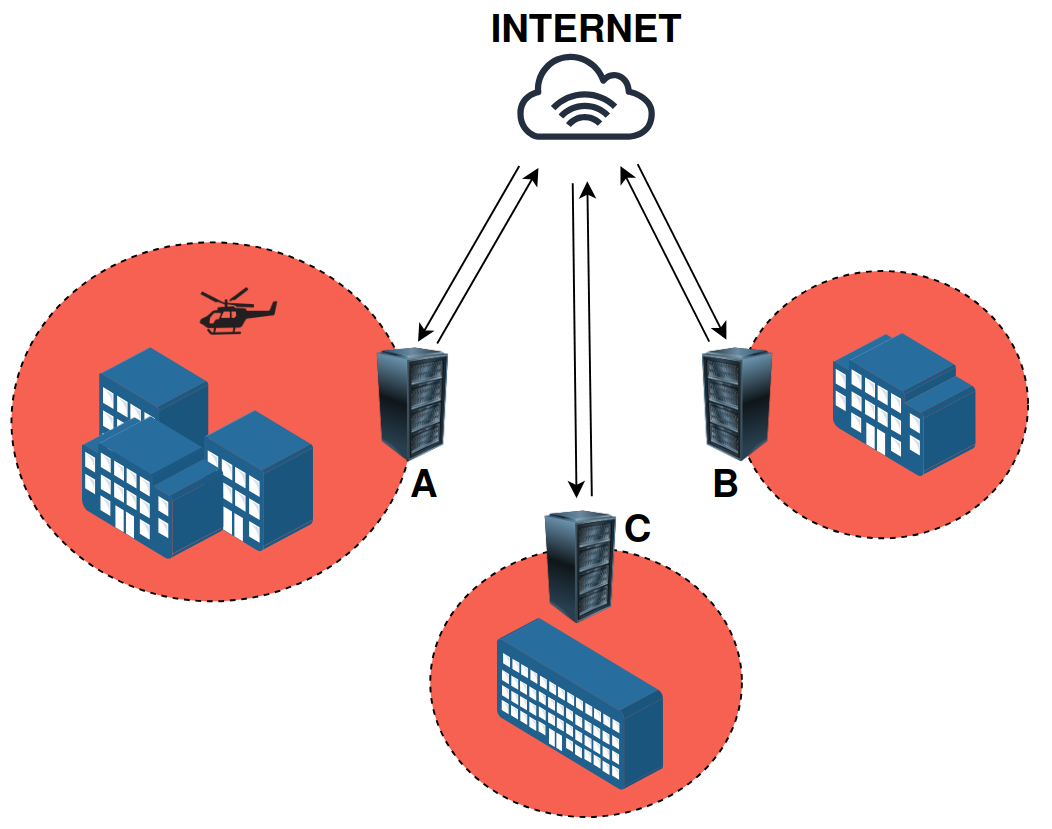
\includegraphics[width=0.75\textwidth]{images/conops.png}
                \caption{\centering Esquema simplificado de operación del sistema.}
            \end{figure}
        \end{column}
    \end{columns}
    \note{Antes que nada quiero dar un pantallazo general de lo que se trata este proyecto. ¿A que nos referimos con sistema de comunicaciones seguras? Se trata del desarrollo de un dispositivo encriptador destinado a asegurar las comunicaciones entre sitios, es decir, que permita establecer una red privada virtual o VPN entre estos sitios.
    En la figura se puede ver un esquema simplificado de la operación del sistema. Estos dispositivos hacen de interfaz entre dos dominios, el rojo, que contiene información no cifrada, y el negro, que es la parte externa, donde la información se encuentra cifrada.
    }
\end{frame}

\begin{frame}{Motivación}
    \begin{itemize}
        \item Abordaje novedoso a las soluciones de encriptación de redes.
        \item Necesidad de una solución propia y auditable.
    \end{itemize}

    \note{Este proyecto surge como una posibilidad de abordar una solución de encriptación de redes de datos con un enfoque novedoso como es la segmentación virtual de dominios. 
    Además, es importante contar con una solución propia, cuyo desarrollo y mantenimiento no dependa de terceros y pueda ser auditada visto casos como el de Crypto AG, una empresa proveedora de equipos de cifrado con backdoors, que por mucho tiempo fue, en secreto, propiedad de entidades gubernamentales.}
\end{frame}

\begin{frame}{Objetivos}
    \begin{itemize}
        \item Validar la viabilidad de realizar segmentación de dominios basada en hipervisores.
        \item Realizar una prueba de concepto del enfoque propuesto.
        \item Implementar una propuesta de solución auditable y documentada.
    \end{itemize}
    \note{Respecto a los objetivos de este proyecto se plantean estos tres puntos. El primero, validar si es viable realizar segmentación virtual de dominios, responde al ¿para qué? del proyecto.
    Los otros objetivos se corresponden con la solución propuesta, el ¿qué? de este proyecto. Lo que se plantea es obtener un encriptador funcional, completamente auditable y documentado.}
\end{frame}


\section{Revisión bibliográfica}
\note{Quiero arrancar con una revisión de algunos conceptos que nos introducen a los sistemas de comunicaciones seguros y que permiten comprender que se busca como propuesta de solución.}

\begin{frame}{Tríada CID}
    \begin{columns}
        \begin{column}{0.5\textwidth}
            \begin{figure}
                \centering
                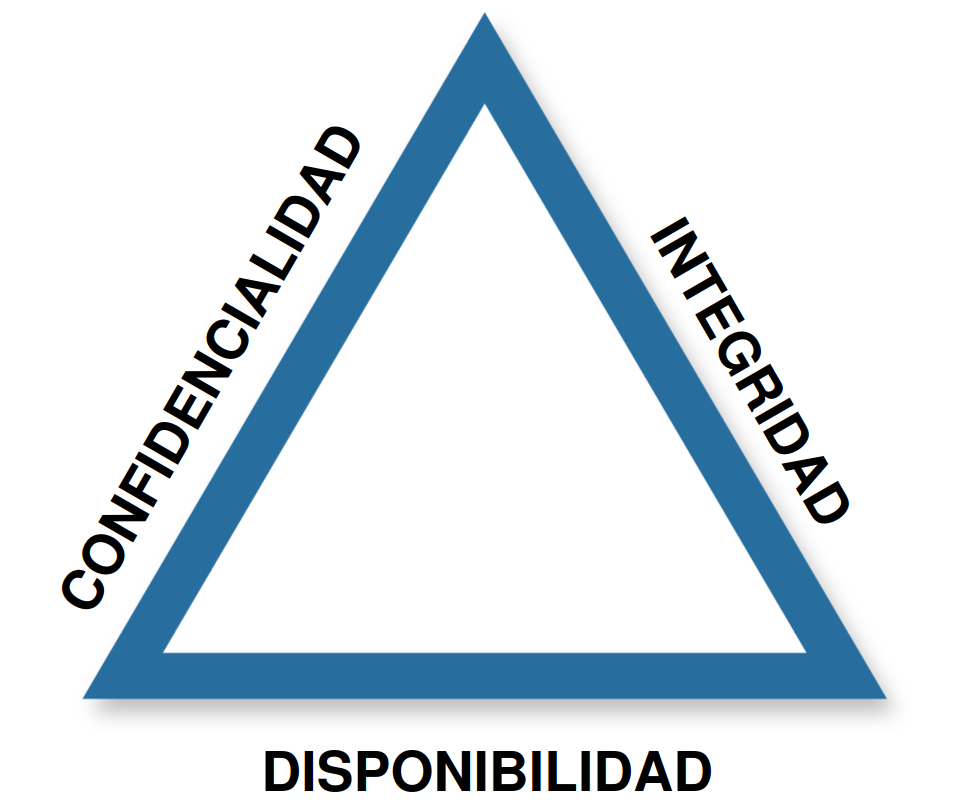
\includegraphics[width=0.9\textwidth]{images/cia.png}
                \caption{Modelo CID.}
            \end{figure}
        \end{column}
    \end{columns}
    \note{La triada CID es un modelo que constituye la base para el diseño de sistemas de seguridad. Se compone de estos tres conceptos fundamentales.

    La confidencialidad implica garantizar que los datos no sean accesibles por usuarios no autorizados. Los esfuerzos en esta área se centran en los métodos de encriptación.
    
    La integridad asegura la autenticidad de los datos, es decir, que estos estén libres de alteraciones. Aqui se pueden mencionar el uso de hashes o firmas digitales.
    
    La disponibilidad garantiza que los datos sean accesibles cuando se los necesite. Un sistema débil en este aspecto puede ser víctima de ataques de denegación de servicio, por ejemplo. Para esto se refuerza el sistema incluyendo redundancia y algoritmos de detección de ataques.}

\end{frame}

\begin{frame}{Encriptación simétrica}
    \begin{columns}
        \begin{column}{0.4\textwidth}
            \begin{itemize}
                \item Clave única.
                \item Requiere un canal seguro para el intercambio de la clave.
                \item La confidencialidad y autenticación dependen tanto de A como de B.
                \item Método eficiente.

            \end{itemize}
        \end{column}
        \begin{column}{0.45\textwidth}
            \begin{figure}
                \centering
                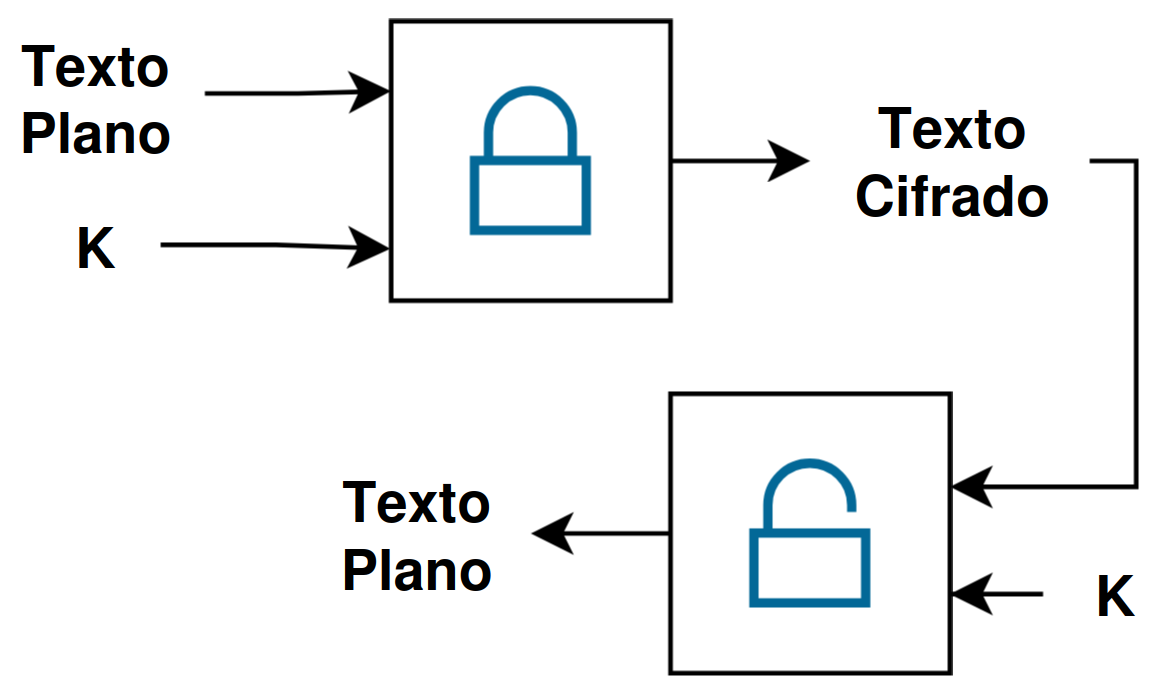
\includegraphics[width=\textwidth]{images/simetric.png}
                \caption{\centering Esquema simplificado de la encriptación simétrica.} 
            \end{figure}
        \end{column}
    \end{columns}
    \note{
    La encriptación simétrica es un método que utiliza una clave única para encriptar y desencriptar la información. En la figura esquematicé el proceso de encriptado y desencriptado de texto, vemos que se utiliza esta clave K en ambos procesos, lo que implica que tanto A como B deben conocer esta clave para poder comunicarse. Un problema surge en el acuerdo de esta clave, por que canales y cómo se transmite, además, si esta clave se ve comprometida por cualquiera de las partes, toda la comunicación queda expuesta.
    Más allá de esto, este es un método muy eficiente, lo que lo hace ideal para encriptar grandes volúmenes de información.
    }
\end{frame}

\begin{frame}{Encriptación asimétrica}
    \begin{columns}
    \begin{column}{0.4\textwidth}
        \begin{itemize}
            \item Par de claves relacionadas.
            \item Mantener la autenticidad y confidencialidad de lo que recibe A depende solo de A.
            \item Mayor costo computacional.

        \end{itemize}
    \end{column}
    \begin{column}{0.50\textwidth}
        \begin{figure}
            \centering
            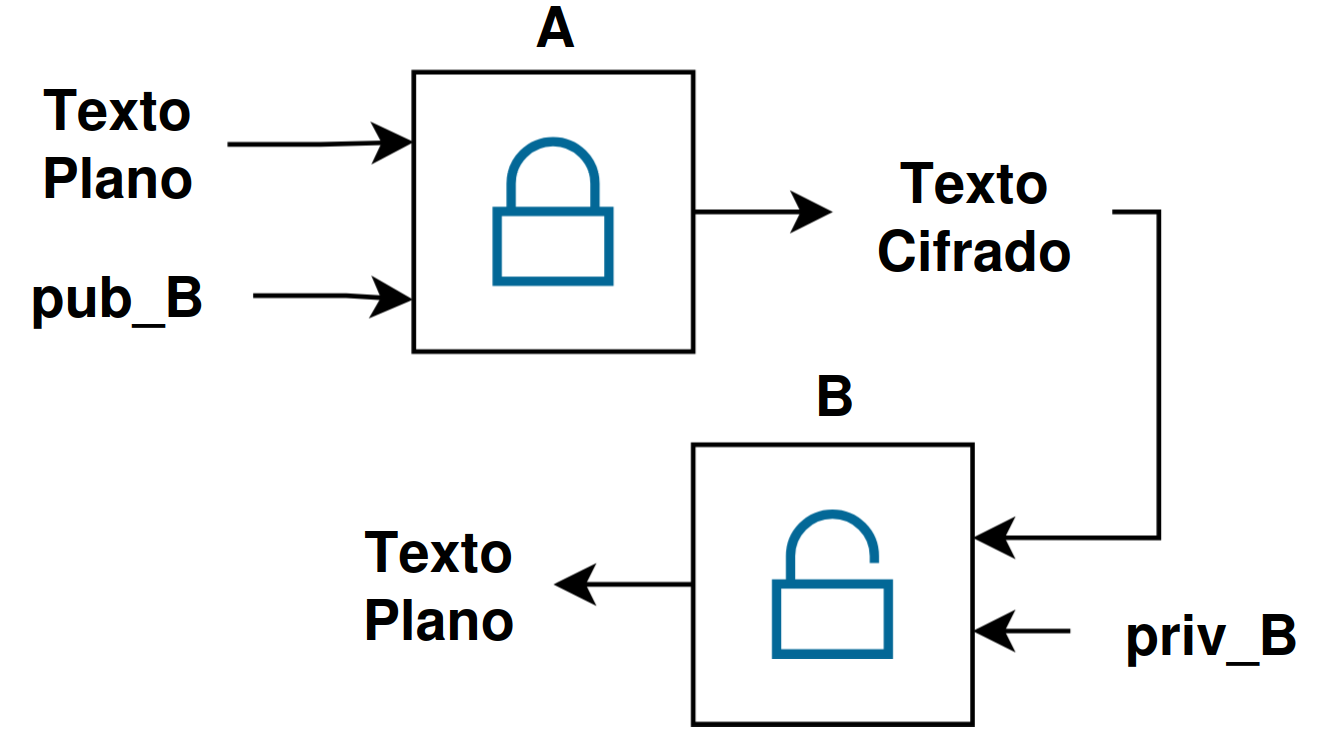
\includegraphics[width=\textwidth]{images/asimetric.png}
            \caption{\centering Esquema simplificado de la encriptación asimétrica.} 
        \end{figure}
    \end{column}
    \end{columns}
    \note{
    La encriptación asimétrica es un método que utiliza un par de claves relacionadas, una clave pública y una privada. La clave pública se puede compartir con cualquier persona, y es utilizada para encriptar, mientras que la clave privada debe mantenerse en secreto y es utilizada para desencriptar. Aquí en la figura se tiene un mensaje de A hacia B, donde A utiliza la clave pública de B. El proceso inverso, un mensaje de B hacia A sería encriptado por B usando la clave pública de A.
    
    Este método además permite que si yo soy A y mi clave privada se ve expuesta, esto solo afecta a la confidencialidad de lo que recibo, puedo seguir enviando mensajes encriptados a B.
    Como contra, este método es más costoso computacionalmente que la encriptación simétrica, no suele utilizarse para grandes volúmenes de información.

    }
\end{frame}


\begin{frame}{Acuerdo de claves Diffie-Hellmann}
    \begin{columns}
        \begin{column}{0.4\textwidth}
            \begin{itemize}
                \item Método para generar una clave compartida sin intercambio directo.
                \item Mitiga un problema de la encriptación simétrica.
                \item No resuelve el problema de autenticación.
            \end{itemize}
        \end{column}
        \begin{column}{0.6\textwidth}
            \begin{figure}
                \centering
                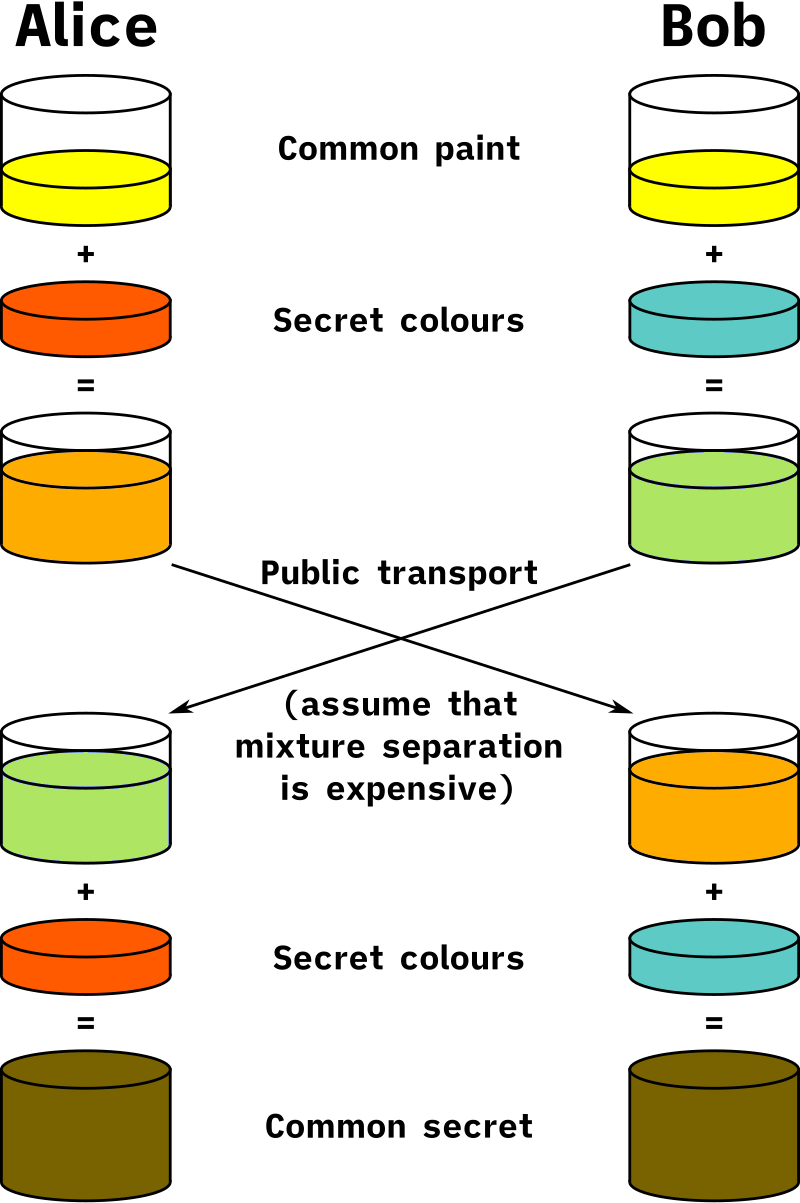
\includegraphics[width=0.45\textwidth]{images/Diffie-Hellman_Key_Exchange.png}
                \caption{\centering Método Diffie-Hellmann simplificado.} 
            \end{figure}
        \end{column}
    \end{columns}
    \note{El acuerdo de claves Diffie-Hellmann es un método para generar una clave compartida sobre un canal inseguro sin necesidad de intercambiarla directamente. De esta forma se mitiga el problema de la encriptación simétrica, que es la necesidad de un canal seguro para el intercambio de claves. 

    Este método se basa en la dificultad matemática del problema del logaritmo discreto en números grandes. Por lo general, los protocolos utilizados utilizan claves de 32 a 56 bytes. 
    
    Este esquema simplificado con pinturas representa el proceso de acuerdo de claves Diffie-Hellmann. A y B generan claves privadas y públicas, y luego intercambian las claves públicas. A partir de las claves públicas de A y B y sus claves privadas propias, cada uno puede obtener la misma clave como resultado.}

\end{frame}

\begin{frame}{Arquitectura red/black}
    \begin{columns}
        \begin{column}{0.4\textwidth}
            \begin{itemize}
                \item Lineamientos para identificar y separar correctamente dominios de información.

            \end{itemize}
        \end{column}
        \begin{column}{0.6\textwidth}
            \begin{figure}
                \centering
                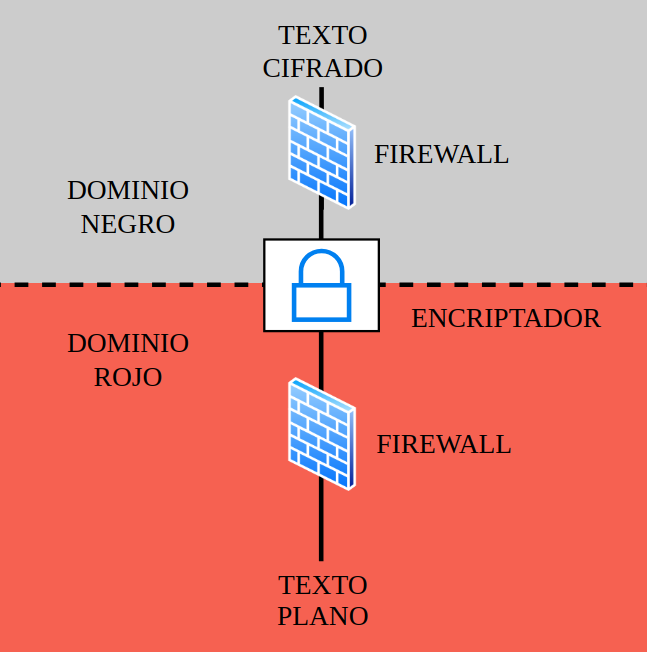
\includegraphics[width=0.58\textwidth]{images/NSA_Red-Gray-Black_diagram.png}
                \caption{Esquema simplificado dominios red/black.} 
            \end{figure}
        \end{column}
    \end{columns}

    \note{El concepto de arquitectura red/black representa la separación de los dominios que contienen texto plano no cifrado de aquellos que contienen texto cifrado.
    Adoptar esta metodología permite identificar las interfaces entre dominios y diseñar medidas de seguridad adecuadas para aislarlas correctamente.

    Esta idea de segregación de interfaces surge de las especificaciones militares TEMPEST, que provee lineamientos en el diseño físico de los equipos. Aquí se encuentra el mayor desafío de este proyecto, que es lograr una implementación segura de esta arquitectura en un entorno virtualizado.}
\end{frame}


\begin{frame}{Hipervisores}
    \begin{columns}
        \begin{column}{0.4\textwidth}
            % seL4 - tipo 0 , formalmente probado
            % Ejemplos de aplicación
            % Importante lograr sandboxing de cada dominio
            Software que permite la ejecución de entidades virtuales independientes sobre hardware compartido.
            \vspace{0.5cm}
            \begin{itemize}
                \item Tipo 1: ejecución sobre hardware. % seL4
                \item Tipo 2: ejecución sobre un sistema operativo. % VirtualBox
            
            % Acá lo importante es asegurar que cada dominio tenga acceso solo a los recursos que necesita y no pueda sobrepasar los límites de su sandbox.

            % Mencionar que seL4 es un hipervisor tipo 1, que cumple con propiedades interesantes para su utilización en sistemas críticos como al que se apunta. Esta formalmente probado, es auditable (open source) y está diseñado para ser seguro sin comprometer el rendimiento.  
            \end{itemize}
        \end{column}

        \begin{column}{0.4\textwidth}
            \begin{figure}
                \centering
                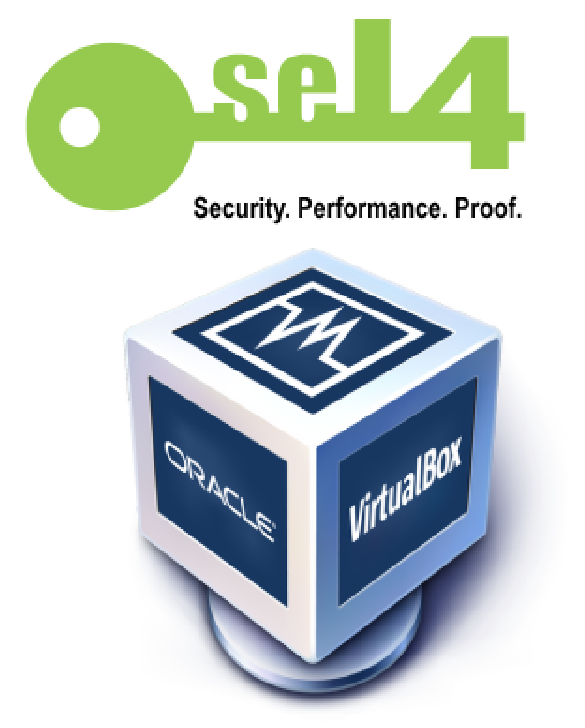
\includegraphics[width=0.7\textwidth]{images/hyperv.png}
                \caption{Ejemplo de hipervisores.} 
            \end{figure}
        \end{column}
    \end{columns}
    \note{Un hipervisor es un software que permite la ejecución y administración de máquinas virtuales sobre un hardware compartido. Gestiona los recursos de hardware y asegura el aislamiento entre las máquinas virtuales fuera de sus interfaces de comunicación. 

    Un hipervisor tipo 1 se ejecuta directamente sobre el hardware, sin necesidad de un sistema operativo intermediario. Ofrece mayor rendimiento y seguridad a costa de mayor complejidad de implementación. Un ejemplo de este tipo de hipervisor es seL4, el cual describiré más adelante.
    
    Un hipervisor tipo 2 se ejecuta sobre un sistema operativo, es más versátil respecto a su implementación. Un ejemplo de este tipo de hipervisor es VirtualBox.}

\end{frame}

\section{Desarrollo}

\begin{frame}{Plan de trabajo}
    \begin{figure}
        \centering
        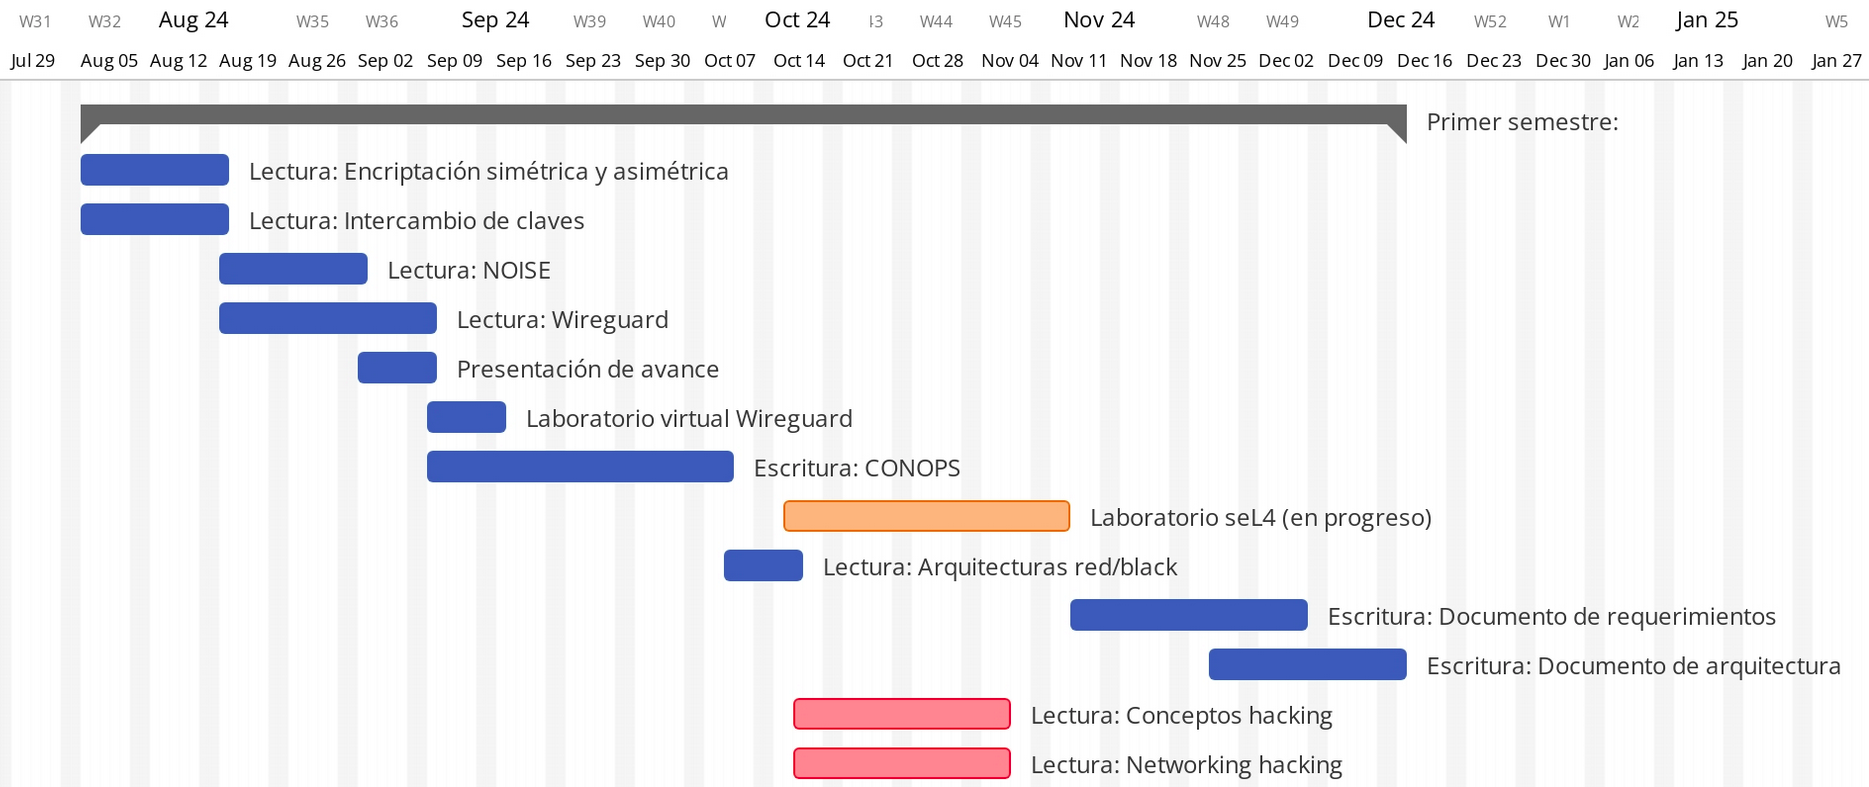
\includegraphics[width=0.96\textwidth]{images/plan.png}
        \caption{Plan de trabajo del primer semestre de proyecto.}
    \end{figure}
    \note{
    Quiero presentar antes que nada lo que fue el primer paso en este proyecto, que fue realizar el plan de trabajo del semestre. Esto me permitió mantener una metodología de trabajo ordenada en lo que es el proyecto. 
    
    Algunas tareas involucraron la lectura como introducción a los conceptos necesarios para comprender el fin del proyecto y otras que permitieron aprender de forma práctica sobre las tecnologías a utilizar. También hay cierta documentación pensada como entregables que consideramos importante para enmarcar la propuesta de solución.
    
    En azul están marcadas las tareas que ya fueron completadas, en rojo las que quedaron pendientes para el segundo semestre.
    }
\end{frame}

\subsection{Propuesta de solución}
\begin{frame}{Método ARCADIA}
    \begin{figure}
        \centering
        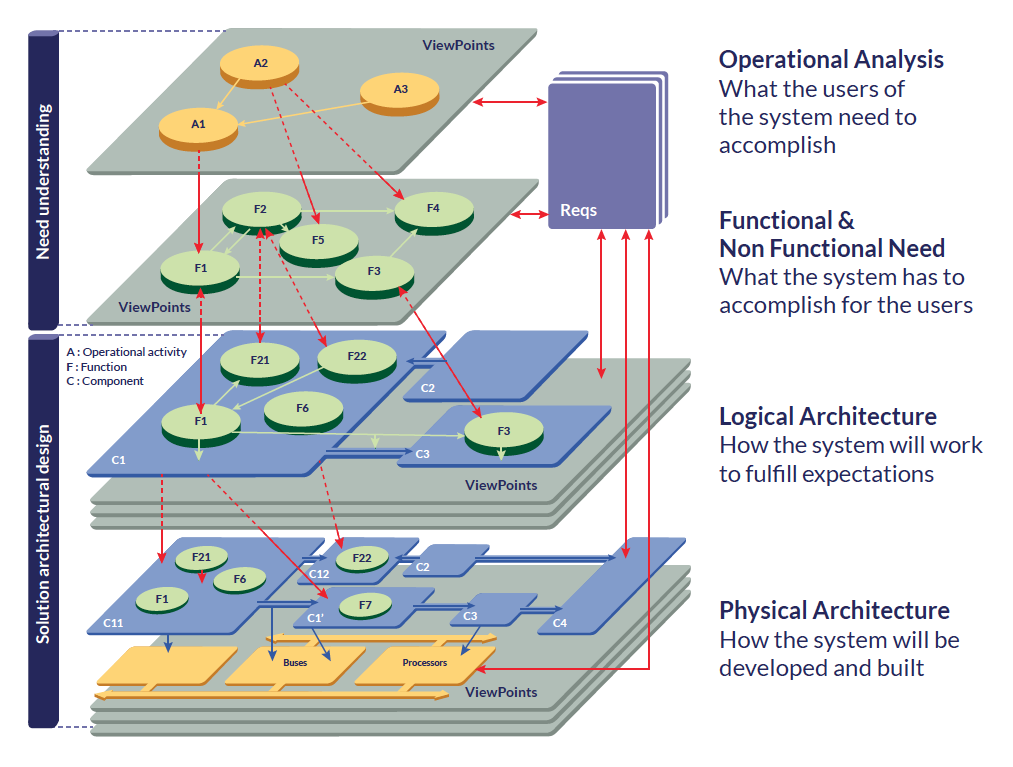
\includegraphics[width=0.58\textwidth]{images/arcadia.png}
        \caption{Desglose del método adoptado.}
    \end{figure}
    \note{Quiero presentar brevemente la forma de trabajo que adoptamos para la elaboración de la propuesta de solución. El método ARCADIA se basa en la identificación de los requerimientos del usuario y la definición de los objetivos del sistema.

    Se trabajó primero en entender las necesidades del usuario, esto es la capa superior de la figura, y comprende el análisis operacional. Luego definimos los requerimientos del sistema como las funciones que debe realizar el sistema para cumplir estas necesidades. Ya con esto documentado se puede abordar el diseño de la solución.
    
    Si bien ya recorrimos todas etapas a lo largo del semestre, el diseño de la solución no está completo, y es probable que se identifiquen más necesidades, requerimientos a medida que se avance en el proyecto. Esto es más bien un proceso iterativo entre estas etapas, por lo que consideramos importante documentar cada necesidad, requerimiento y decisión de diseño.}

\end{frame}


\begin{frame}{Análisis operacional}
    \begin{columns}
        \begin{column}{0.38\textwidth}
            \begin{itemize}
            \item Definición del problema.
            \item Planteo de las necesidades del usuario.
            \item Alcance de la solución.
            \item Concepto de operaciones.
            \end{itemize}

            % \begin{figure} % QR?
            %     \centering
            %     \href{https://github.com/adl09/ADL_public/blob/main/CONOPS.pdf}{
\includegraphics[width=0.5\textwidth]{images/CONOPS_QR.png}}
            %     \caption{Concepto de operaciones.}
            % \end{figure}
            
        \end{column}

        \begin{column}{0.45\textwidth}
            \begin{figure}
                \centering
                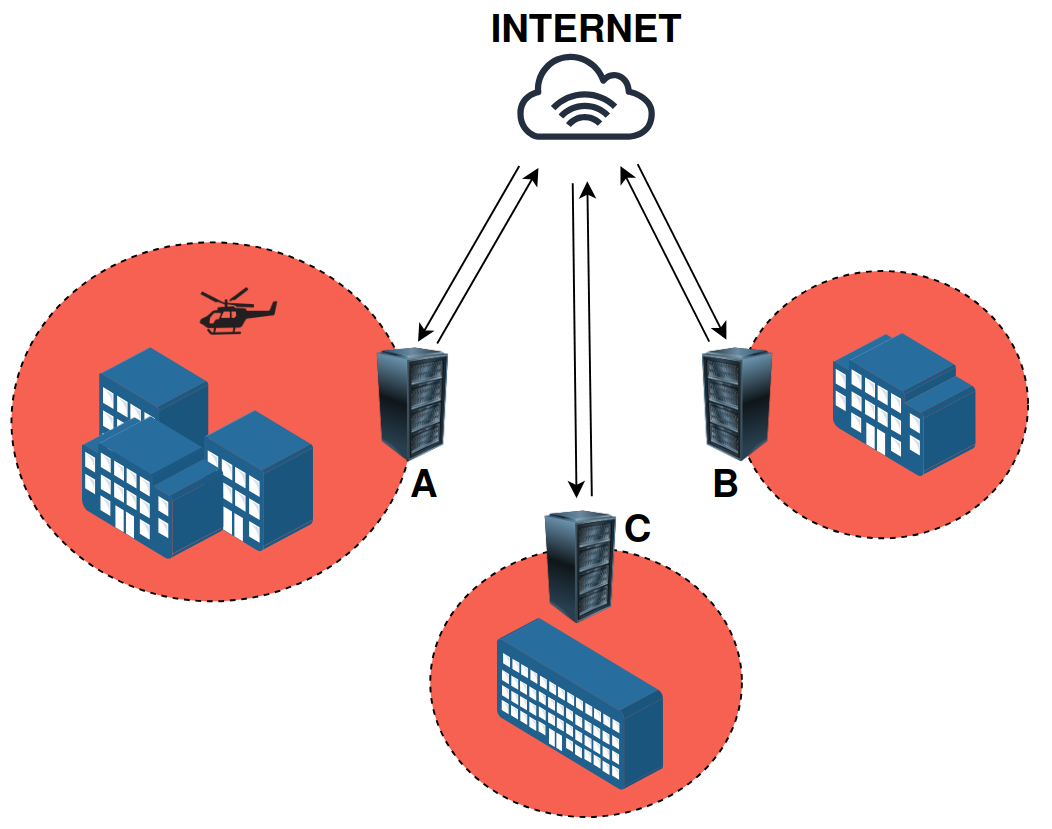
\includegraphics[width=\textwidth]{images/conops.png}
                \caption{\centering Esquema simplificado del sistema propuesto.} 
            \end{figure}
        \end{column}
    \end{columns}

    \note{Partiendo de la primer capa del modelo, planteamos el concepto de operaciones del sistema, que se encuentra documentado y puede accederse a una copia desde este QR.

    Esta etapa involucró definir el problema y el contexto en el que se desarrolla la solución. Se manifiestan las suposiciones y limitaciones del sistema propuesto, como puede ser el análisis de encriptación en capa física respecto a hacerlo en capa de red, por ejemplo.
    
    Se documentó también el alcance de la solución, que es la definición de los límites del sistema y las funciones que debe cumplir, sin profundizar en cómo se va a lograr esto.
    
    Este es un esquema simplificado del sistema propuesto. Cada nodo de la red segura se comunica con los demás a través de una conexión a Internet.}

\end{frame}

\begin{frame}{Modos de operación}
    \begin{columns}
        \begin{column}{0.45\textwidth}
            \begin{figure}
                \centering
                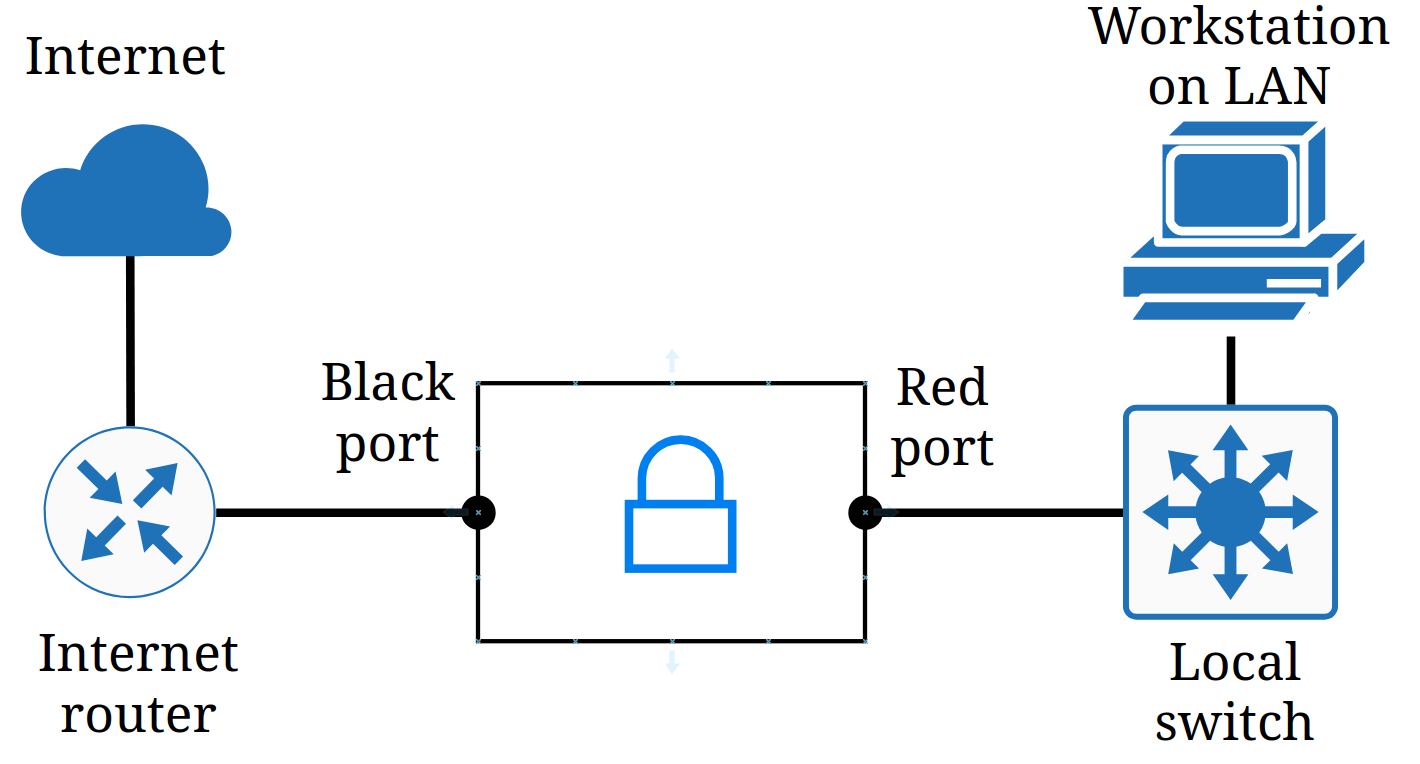
\includegraphics[width=\textwidth]{images/smallmode_conops.png}
                \caption{\centering Despliegue en sitio sin infraestructura de red.} 
            \end{figure}
        \end{column}

        \begin{column}{0.45\textwidth}
            \vspace{4mm}
            \begin{figure}
                \centering
                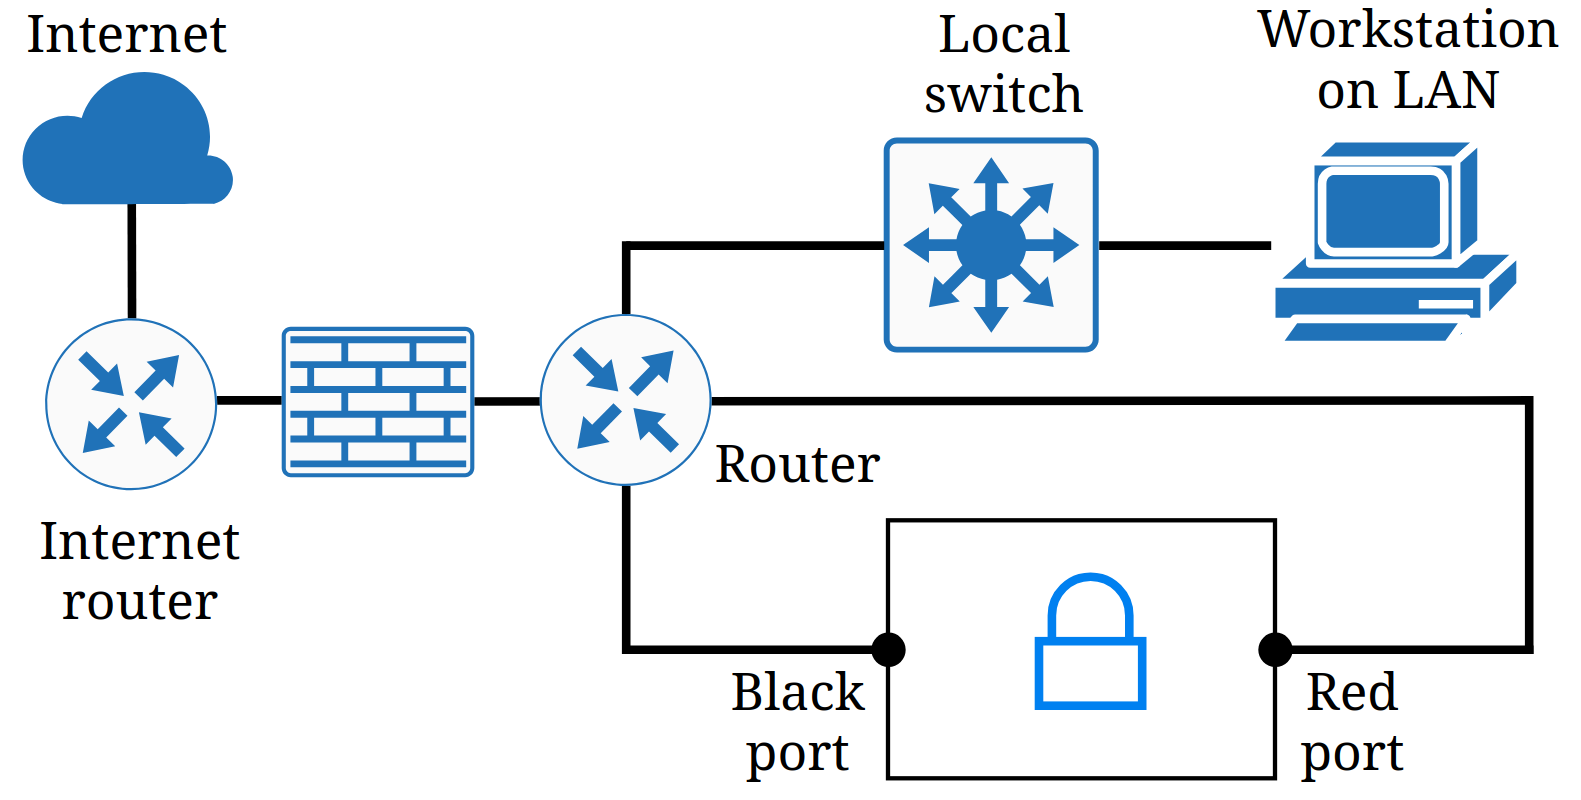
\includegraphics[width=\textwidth]{images/bigmode_conops.png}
                \caption{\centering Despliegue en sitio con infraestructura de red.} 
            \end{figure}
        \end{column}
    \end{columns}

    \note{Teniendo en cuenta una configuración de hardware genérica donde se implementará la solución se plantea la posibilidad de dos modos de operación.
    Se considera nodo pequeño a un sitio con poco tráfico, en el que el hardware del encriptador es capaz de direccionar todo el tráfico de la red según su destino sea Internet u otro nodo de la red segura.
    Si se trata de un nodo grande, puede que el hardware del encriptador no sea capaz de direccionar todo el tráfico. En este caso es necesario un router que cumpla esta función, de manera que solo el tráfico destinado a otro nodo red segura pasa por el encriptador.}

\end{frame}


\begin{frame}{Requerimientos}
    \begin{itemize}
        \item \textbf{Funcionales}: renovación de claves, manejo de ataques DoS.
        \item \textbf{Rendimiento}: tasa de transferencia, número de nodos.
        \item \textbf{Interfaz}: administración, interfaces físicas.
        \item Documento de requerimientos.
    \end{itemize}

    % \begin{figure} 
    %     \href{https://github.com/adl09/ADL_public/blob/main/Requerimientos.pdf}{
\includegraphics[width=0.2\textwidth]{images/Requerimientos_QR.png}}
    %     \caption{Documento de requerimientos.}
    % \end{figure}

    \note{En un nivel menor de abstracción se definieron los requerimientos del sistema, estos son las cosas que el sistema debe hacer para cumplir con las necesidades planteadas en el concepto de operaciones. 
    Como ejemplos están el tiempo asociado a la renovación de claves que maneja el encriptador, la tasa máxima de transferencia entre nodos y las interfaces de administración del encriptador.
    Estos requerimientos se documentaron y pueden accederse a una copia desde este QR.
    }
\end{frame}

% ACÁ YA ENTRAMOS EN EL DOMINIO DE LA SOLUCIÓN PROPUESTA
% COMO SE VAN A CUMPLIR LOS REQUERIMIENTOS DEL SISTEMA

\begin{frame}{Arquitectura lógica}
    \begin{columns}
        \begin{column}{0.4\textwidth}
            \begin{itemize}
            \item Uso de un hipervisor con \\ tres máquinas virtuales independientes.
            \item Documento de arquitectura.
            % indicar que hace cada máquina A,B,C
            % De momento los firewalls implementados solo involucran un filtrado de paquetes con iptables.
            \end{itemize}

            % \begin{figure} % QR?
            %     \centering
            %     \href{https://github.com/adl09/ADL_public/blob/main/Arquitectura.pdf}{
\includegraphics[width=0.5\textwidth]{images/Arquitectura_QR.png}
            %     }
            %     \caption{\centering Documento de arquitectura.}
            % \end{figure}
        \end{column}

        \begin{column}{0.6\textwidth}
            \begin{figure}
                \centering
                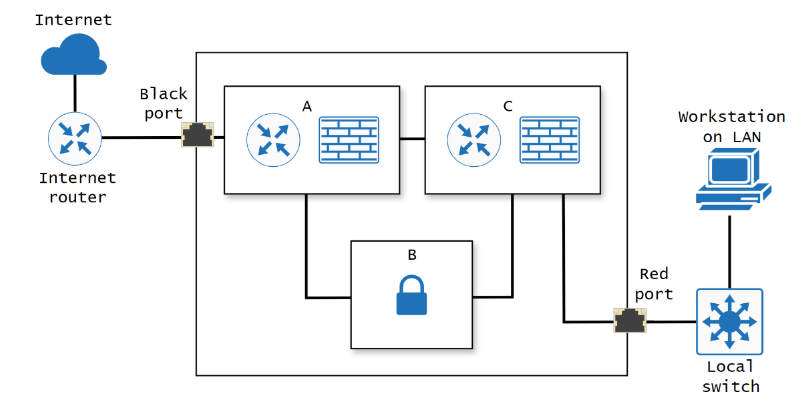
\includegraphics[width=\textwidth]{images/arquitectura.png}
                \caption{Arquitectura lógica de la solución propuesta.} 
            \end{figure}
            % Hacer una figura decente onda esto
        \end{column}
    \end{columns}
    \note{Como última etapa queda proponer una arquitectura lógica para hacer cumplir los requerimientos del sistema, aquí ya estamos pensando sobre la solución. 

    Se planteó el uso de un hipervisor con tres máquinas virtuales independientes y aislados salvo por ciertas interfaces de comunicación definidas. 

    En esta etapa también se defieron las tecnologías a usar para implementar esta arquitectura.
    }

\end{frame}


\begin{frame}{Tecnologías a usar}
    % NOISE
    % WIREGUARD
    % seL4
    % Destacar que todas son open-source.
    \begin{columns}[T]
        \begin{column}{0.33\textwidth}
    \onslide<1->{
            \begin{center}
                \textbf{NOISE}
            \end{center}
            \begin{itemize}
                \item Framework para el desarrollo de protocolos seguros.
            \end{itemize}
        
    }
        \end{column}
    

        \begin{column}{0.33\textwidth}
    \onslide<2->{
            \begin{center}
                \textbf{Wireguard}
            \end{center}
            \begin{itemize}
                \item Software VPN.
                \item Opera a nivel de \\ capa de red.
                \item Base de código reducida.
            \end{itemize}
     }
        \end{column}
        \begin{column}{0.33\textwidth}
            \onslide<3->{

            \begin{center}
                \textbf{seL4}
            \end{center}
            \begin{itemize}
                \item Microkernel.
                \item Hipervisor tipo 1.
                \item Formalmente probado.
            \end{itemize}
    }
        \end{column}
    \end{columns}

    \note{
    Para implementar la propuesta de solución se plantea el uso de tres tecnologías open-source.
        En primer lugar está NOISE, un framework para el desarrollo de protocolos seguros basado en el método Diffie-Hellmann que cuenta con una serie de protocolos formalmente probados, aplicaciones como WhatsApp son un ejemplo de uso de este framework en el cifrado de mensajería.
        
        Wireguard es un software que permite la creación de VPNs de forma sencilla y segura. Utiliza protocolos derivados del framework NOISE para el establecimiento de conexiones.
        Opera a nivel de capa 3 del modelo OSI. Un aspecto importante es que su código fuente es reducido, aproximadamente 4000 líneas de código, lo cual ayuda a reducir la superficie de ataque.
        
        seL4 es un microkernel diseñado para ser seguro, eficiente y confiable. Se ejecuta directamente sobre hardware con capacidad de funcionar como hipervisor de tipo 1. Cuenta con verificación formal de su funcionamiento, esto quiere decir que se demostró matemáticamente que su implementación cumple con sus especificaciones de diseño. Una de estas especificaciones es la aislación entre componentes.
        En resumen, tenemos un hipervisor en donde la aislación de procesos entre máquinas virtuales está garantizada, lo cuál es crítico en nuestro sistema.

    }

\end{frame}

\subsection{Laboratorios virtuales}
\note{
}

\begin{frame}{Laboratorio virtual - Wireguard}
    \begin{columns}
        \begin{column}{0.4\textwidth}
            \begin{itemize}
                \item Fundamentos de redes.
                \item Utilización de Wireguard.
            \end{itemize}
        \end{column}
        \begin{column}{0.55\textwidth}
            \begin{figure}
                \centering
                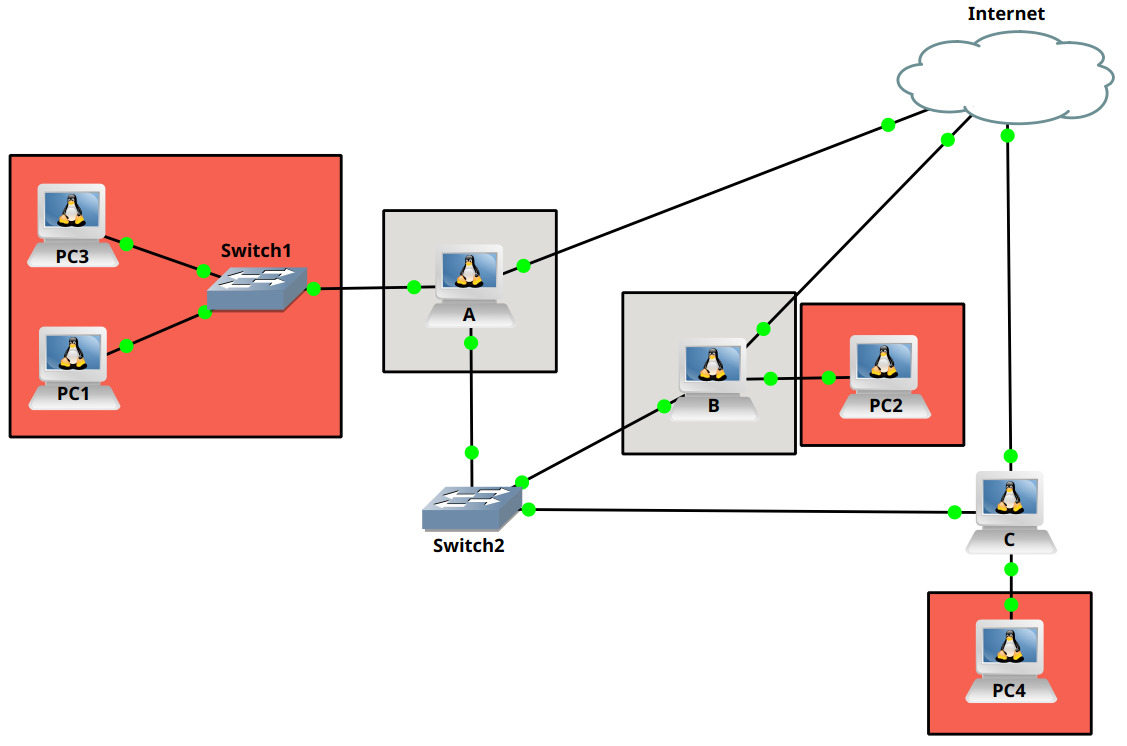
\includegraphics[width=\textwidth]{images/gns3_1.png}
                \caption{Primeras pruebas con Wireguard en GNS3.}
            \end{figure}
        \end{column}
    \end{columns}
    \note{
        Sobre GNS3, un hipervisor de tipo 2 se implementó una red como la de la imagen utilizando máquinas virtuales Linux. Se configuraron dos nodos, A y B, a modo de encriptadores usando Wireguard. Analizando el tráfico de la red se verificó que la comunicación entre los nodos esté encriptada y que el tráfico con destino a Internet se direccione por fuera del túnel VPN.
    }
\end{frame}

\begin{frame}{Laboratorio virtual - Wireguard}
    \begin{figure}
        \centering
        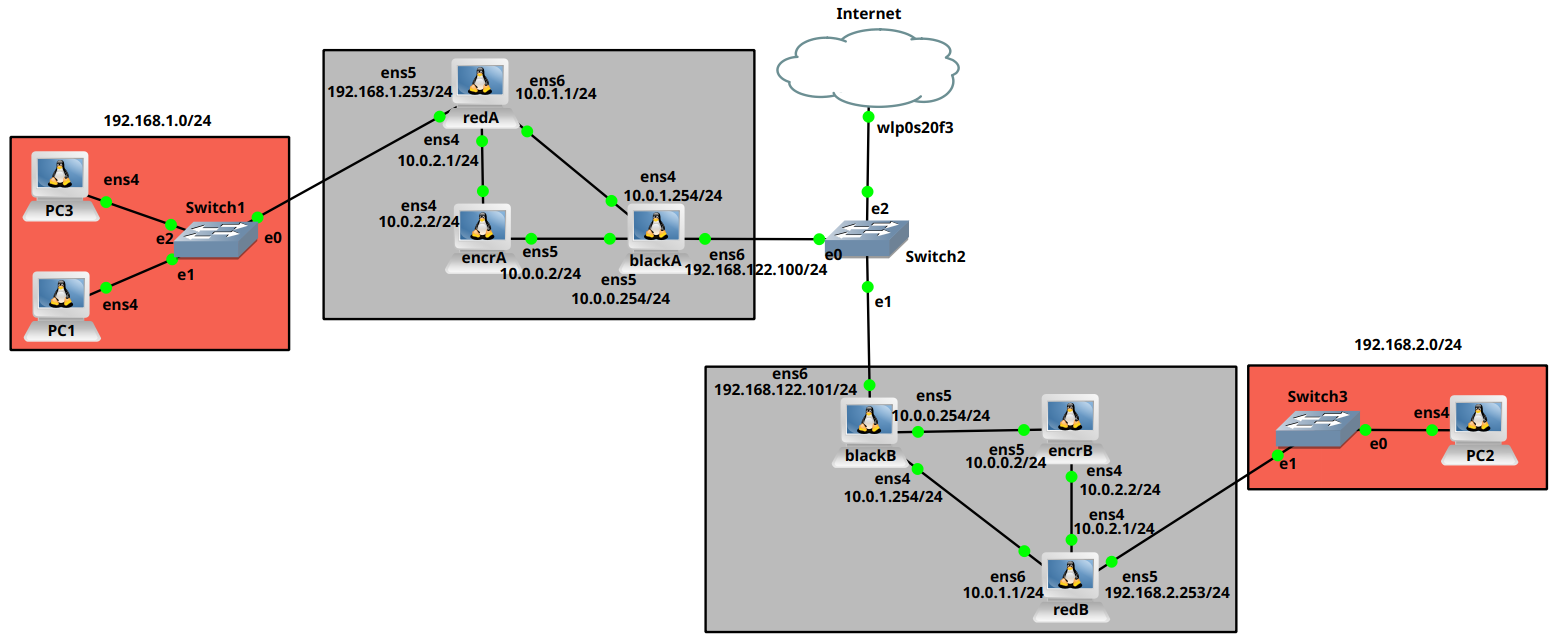
\includegraphics[width=0.95\textwidth]{images/gns3_2.png}
        \caption{Implementación de la propuesta de solución en GNS3.} 
    \end{figure}
    \note{
        También se verificó esto sobre una red donde implementamos la arquitectura propuesta para los encriptadores utilizando tres máquinas virtuales independientes. Dos actuando como routers y una como encriptador.
        En este caso los paquetes con destino otro nodo de la red segura llegan a "router", se encriptan en "red" y salen a Internet a través de la interfaz física de "black".
        El tráfico que no debe ser encriptado se dirige desde "router" directamente a "black".
    }
\end{frame}


% \begin{frame}{Laboratorio virtual - seL4}
%     \begin{itemize}
%         \item Introducción a seL4.
%         \item Introducción al desarrollo de software utilizando contenedores.
%     \end{itemize}
%     \note{
%         Respecto a seL4 se realizaron unos pocos tutoriales introductorios propios de la documentación oficial, que si bien fueron no mucho más que instalar el entorno en mi PC y correr un Hello World, fueron útiles para familiarizarse con el entorno de desarrollo. 

%         Todo esto se implementó usando contenedores Docker, algo muy útil para mantener un entorno de desarrollo limpio y reproducible en otros equipos.

%     }
% \end{frame}


\section{Conclusiones}
\begin{frame}{Resumen}
    \begin{columns}
        \begin{column}{0.9\textwidth}
            \begin{itemize}
                \item Introducción a los conceptos de sistemas de comunicaciones seguras.
                \item Elaboración e implementación simulada de una propuesta de solución.
                \item Familiarización con las tecnologías a utilizar.
            \end{itemize}
        \end{column}
    \end{columns}

    % Agrego tres figuras en 3 columnas
    % \begin{columns}
    %     \begin{column}{0.33\textwidth}
    %         \begin{figure} % QR?
    %                 \centering
    %                 \href{https://github.com/adl09/ADL_public/blob/main/CONOPS.pdf}{
\includegraphics[width=0.5\textwidth]{images/CONOPS_QR.png}}
    %                 \caption{\centering Concepto de operaciones.}
    %             \end{figure}
    %     \end{column}
    %     \begin{column}{0.33\textwidth}
    %             \begin{figure} 
    %                 \href{https://github.com/adl09/ADL_public/blob/main/Requerimientos.pdf}{
\includegraphics[width=0.5\textwidth]{images/Requerimientos_QR.png}}
    %                 \caption{\centering Documento de requerimientos.}
    %             \end{figure}
    %     \end{column}
    %     \begin{column}{0.33\textwidth}
    %         \begin{figure} % QR?
    %             \centering
    %             \href{https://github.com/adl09/ADL_public/blob/main/Arquitectura.pdf}{
\includegraphics[width=0.5\textwidth]{images/Arquitectura_QR.png}
    %             }
    %             \caption{\centering Documento de arquitectura.}
    %         \end{figure}
    %     \end{column}
    % \end{columns}

    \note{En resumen, se estudiaron conceptos de sistemas de comunicaciones seguras y redes de datos. Se elaboró una arquitectura para la propuesta de solución y se la implementó de forma simulada en GNS3. Y por último, la realización del laboratorio virtual y los tutoriales permitieron familiarizarse con Wireguard y seL4, las tecnologías a utilizar en la propuesta de solución.}
\end{frame}

\begin{frame}{Trabajo a futuro}
    \begin{columns}
        \begin{column}{0.9\textwidth}
            \begin{itemize}
                \item Reformular la implementación simulada del encriptador en seL4 \\ y posteriormente implementarlo en hardware.
                \item Adquirir conceptos de hacking para realimentar el diseño de la solución.
                \item Continuar con la documentación del proyecto.
            \end{itemize}
        \end{column}
    \end{columns}


    \note{
        Como trabajo a futuro se plantea continuar con la implementación virtual de la arquitectura propuesta en seL4 y posteriormente en hardware corriendo seL4.
        También falta adquirir conceptos que nos permitan realimentar el diseño de la solución.
        Continuar con este proceso iterativo que es la documentación del proyecto.

    }
\end{frame}

\begin{frame}
    \begin{center}
        \Huge ¡Muchas gracias! \\
        \Huge ¿Preguntas?
    \end{center}
\end{frame}

% FIN

\end{document}